\documentclass[11pt]{article}
\usepackage[margin=1in]{geometry}
\usepackage{booktabs}
\usepackage{xcolor}
\usepackage{amsmath}
\usepackage{float}
\usepackage{graphicx}
\usepackage{hyperref}

\hypersetup{colorlinks=true, linkcolor=blue!60!black}

\newcommand{\win}[1]{\textcolor{green!50!black}{\textbf{#1}}}
\newcommand{\bad}[1]{\textcolor{red!70!black}{#1}}

\title{Routing Scheme Evaluation Results}
\author{Autonomous Networks Research Group (ANRG)\\University of Southern California}
\date{}

\begin{document}
\maketitle
\tableofcontents
\newpage

%======================================================================
\section{Evaluation Setup}

\begin{table}[H]
\centering
\begin{tabular}{ll}
\toprule
\textbf{Parameter} & \textbf{Value} \\
\midrule
Seeds per combo        & 30 (seeds 1--30); values are mean makespan \\
Schedulers             & HEFT: calibrated to runtime routing model \\
                       & HEFT-1: direct-link BW; 0.001\,MB/s for non-adjacent \\
                       & HEFT-2: widest-path BW for all pairs (fixed) \\
Routing schemes        & W, S, SH, GS, GC, GB, GO, GSD, GSD-D \\
Interference model     & \texttt{csma\_bianchi} (802.11ax, 5\,GHz, 20\,MHz) \\
RF parameters          & $P_\text{tx}=20$\,dBm, path-loss exponent $n=3.0$ \\
Grid spacing           & 40\,m; adjacent-link PHY rate $\approx8.6$\,MB/s \\
Compute costs          & 150--1000\,cu (heterogeneous, $\approx6.7\times$ range) \\
Data sizes             & 2--30\,MB (heterogeneous, $15\times$ range) \\
Node capacities        & 80--300\,cu/s (heterogeneous) \\
Total runs             & 3 schedulers $\times$ 9 routing $\times$ 4 experiments $\times$ 30 seeds = 3240 \\
\bottomrule
\end{tabular}
\caption{Evaluation parameters.}
\end{table}

\medskip\noindent
\textbf{HEFT} (calibrated) passes the runtime routing model to HEFT's pairwise
rate matrix, so placement decisions are calibrated to whichever routing scheme
runs at simulation time.  Equals HEFT-2 when paired with \texttt{widest\_path}.

\medskip\noindent
\textbf{HEFT-1} pins 0.001\,MB/s on all non-adjacent pairs regardless of runtime
routing.  Strongly biases placement toward same-node or direct-neighbour assignments.

\medskip\noindent
\textbf{HEFT-2} always uses \texttt{WidestPathRouting} for pairwise BW estimates,
regardless of the runtime routing scheme.

\medskip\noindent
\textbf{SH} (Shortest Hop) minimises hop count, breaking ties by $\sum 1/b_\ell$.
Added alongside S to test whether reducing relay count reduces csma\_bianchi
interference enough to offset lower bottleneck bandwidth.

%======================================================================
\section{Makespan vs.\ Grid Size}

Each point is the \emph{best-routing} mean makespan for that scheduler at
that grid size, averaged over 30 seeds.  Routing scheme labels are annotated
next to each point.

\begin{figure}[H]
\centering
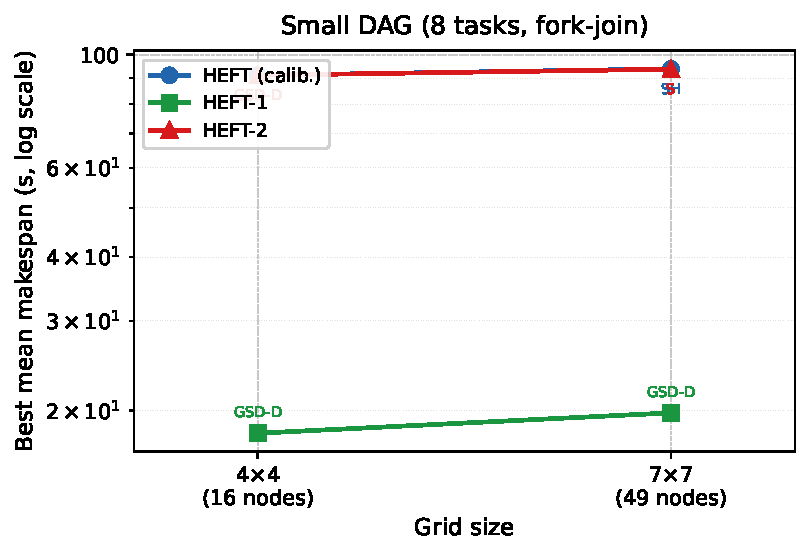
\includegraphics[width=0.72\textwidth]{grid_small.pdf}
\caption{Best-routing mean makespan vs.\ grid size --- Small DAG (8 tasks,
fork-join).  HEFT-1 stays flat near 18--20\,s regardless of grid size; HEFT
and HEFT-2 are nearly identical and rise only marginally from 4$\times$4
to 7$\times$7 ($<$4\%).}
\end{figure}

\begin{figure}[H]
\centering
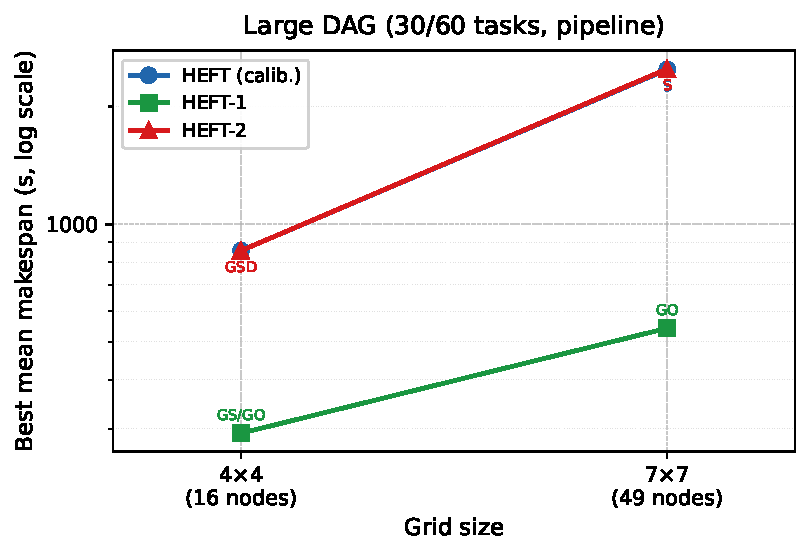
\includegraphics[width=0.72\textwidth]{grid_large.pdf}
\caption{Best-routing mean makespan vs.\ grid size --- Large DAG (30 tasks
on 4$\times$4, 60 tasks on 7$\times$7).  HEFT-1 scales from 292\,s to 542\,s
($1.9\times$); HEFT and HEFT-2 scale from 856\,s to 2490\,s ($2.9\times$),
widening the HEFT-1 advantage from $2.9\times$ to $4.6\times$ as the grid grows.}
\end{figure}

%======================================================================
\section{Full Results Tables}

Mean makespan in seconds, averaged over 30 seeds.
\win{Bold green}: overall experiment winner.
\bad{Red}: worst entry in that column.
$\dagger$: best within that scheduler column.

%----------------------------------------------------------------------
\subsection{$4\times4$ Grid, Small DAG (8 tasks, fork-join, 12 edges)}

\begin{table}[H]
\centering
\small
\begin{tabular}{l r r r}
\toprule
\textbf{Routing} & \textbf{HEFT (s)} & \textbf{HEFT-1 (s)} & \textbf{HEFT-2 (s)} \\
\midrule
W     & \bad{1814.518} &  18.336          & \bad{1814.518} \\
S     &   93.856       &  18.336          &   93.856       \\
SH    &   93.856       &  18.336          &   93.856       \\
GS    &   93.319       &  18.336          &   93.319       \\
GC    &   93.319       &  18.336          &   93.319       \\
GB    &   93.319       &  18.336          &   93.319       \\
GO    &   93.319       &  18.336          &   93.319       \\
GSD   &  140.483       &  18.336          &  140.483       \\
GSD-D &  \textbf{91.134}$^\dagger$ & \win{18.035}$^\dagger$ & \textbf{91.134}$^\dagger$ \\
\midrule
\textit{Best} & \textit{GSD-D 91.134} & \textit{GSD-D 18.035} & \textit{GSD-D 91.134} \\
\bottomrule
\end{tabular}
\caption{$4\times4$ small. HEFT-1 co-locates all 8 tasks on one node; no transfers
occur, so routing is irrelevant (all schemes tie at 18.336\,s). GSD-D gains 0.3\,s via
deferral logic on same-node handoffs. HEFT and HEFT-2 are identical here (both use
widest-path BW when routing=W; for other schemes the 4$\times$4 topology's BW estimates
converge). SH $\equiv$ S throughout: grid paths that minimise $\sum 1/b$ also minimise
hops on this small topology.}
\end{table}

%----------------------------------------------------------------------
\subsection{$4\times4$ Grid, Large DAG (30 tasks, 5-stage pipeline, 48 edges)}

\begin{table}[H]
\centering
\small
\begin{tabular}{l r r r}
\toprule
\textbf{Routing} & \textbf{HEFT (s)} & \textbf{HEFT-1 (s)} & \textbf{HEFT-2 (s)} \\
\midrule
W     & \bad{2383.795} &  497.788          & \bad{2383.795} \\
S     & 1071.723       &  292.425          & 1071.723       \\
SH    & 1071.723       &  292.425          & 1071.723       \\
GS    & 1026.909       &  \textbf{292.091}$^\dagger$ & 1026.909 \\
GC    & 1066.630       &  \textbf{292.091}$^\dagger$ & 1066.630 \\
GB    & 1156.735       &  \textbf{292.091}$^\dagger$ & 1156.735 \\
GO    & 1022.295       &  \textbf{292.091}$^\dagger$ & 1022.295 \\
GSD   & \textbf{855.880}$^\dagger$ & 671.422 & \textbf{855.880}$^\dagger$ \\
GSD-D & 1037.424       &  322.536          & 1037.424       \\
\midrule
\textit{Best} & \textit{GSD 855.880} & \textit{GS/GC/GB/GO \win{292.091}} & \textit{GSD 855.880} \\
\bottomrule
\end{tabular}
\caption{$4\times4$ large. HEFT and HEFT-2 are identical: with 30 tasks all paths
converge regardless of routing calibration. Under HEFT-1, static greedy schemes
(GS/GC/GB/GO) all tie at 292.091\,s---$-41\%$ vs W---by routing direct-neighbour
transfers efficiently. Within the original HEFT, GSD wins at 855.880\,s: calibrated
placement spreads tasks and GSD's runtime congestion avoidance pays off. SH $\equiv$ S
again: min-hop and min-delay paths coincide on this compact grid.}
\end{table}

%----------------------------------------------------------------------
\subsection{$7\times7$ Grid, Small DAG (8 tasks, fork-join, 12 edges)}

\begin{table}[H]
\centering
\small
\begin{tabular}{l r r r}
\toprule
\textbf{Routing} & \textbf{HEFT (s)} & \textbf{HEFT-1 (s)} & \textbf{HEFT-2 (s)} \\
\midrule
W     & \bad{1926.814} &  24.608          & \bad{1926.814} \\
S     &   93.902       &  20.262          &   \textbf{93.696}$^\dagger$ \\
SH    &   \textbf{93.819}$^\dagger$ & 20.262 & 94.067 \\
GS    & 1358.794       &  20.262          & 1309.776 \\
GC    & 1135.942       &  20.262          & 1139.435 \\
GB    & 1597.079       &  20.262          & 1545.814 \\
GO    & 1494.147       &  20.262          & 1542.840 \\
GSD   & 1393.943       &  20.262          & 1459.882 \\
GSD-D & 1512.787       &  \win{19.779}$^\dagger$ & 1338.502 \\
\midrule
\textit{Best} & \textit{SH 93.819} & \textit{GSD-D 19.779} & \textit{S 93.696} \\
\bottomrule
\end{tabular}
\caption{$7\times7$ small. The only experiment where SH and S diverge under HEFT: SH
(93.819\,s) edges out S (93.902\,s) by 0.08\,s---a 0.1\% difference, within noise. Under
HEFT-2, S (93.696\,s) wins. Under HEFT-1 all tasks are co-located; GSD-D wins at 19.779\,s
via deferral. Greedy static schemes under HEFT/HEFT-2 collapse to 1100--1600\,s because
calibrated placement spreads tasks but greedy routing cannot handle the congestion.}
\end{table}

%----------------------------------------------------------------------
\subsection{$7\times7$ Grid, Large DAG (60 tasks, 6-stage pipeline, 102 edges)}

\begin{table}[H]
\centering
\small
\begin{tabular}{l r r r}
\toprule
\textbf{Routing} & \textbf{HEFT (s)} & \textbf{HEFT-1 (s)} & \textbf{HEFT-2 (s)} \\
\midrule
W     & \bad{5695.953} & 1318.190          & \bad{5657.358} \\
S     & \textbf{2487.685}$^\dagger$ & 618.267 & \textbf{2497.366}$^\dagger$ \\
SH    & 2536.137       &  656.054          & 2530.784       \\
GS    & 4295.565       &  660.732          & 4432.067       \\
GC    & 4431.863       &  615.080          & 4468.524       \\
GB    & 4353.115       &  624.117          & 4511.408       \\
GO    & 4439.492       &  \win{542.189}$^\dagger$ & 4361.533 \\
GSD   & 4192.354       & 1278.159          & 4459.398       \\
GSD-D & 4436.056       & 1556.583          & 4474.458       \\
\midrule
\textit{Best} & \textit{S 2487.685} & \textit{GO \win{542.189}} & \textit{S 2497.366} \\
\bottomrule
\end{tabular}
\caption{$7\times7$ large. \textbf{S beats SH} under both HEFT ($-2\%$) and HEFT-1
($-6\%$): on this topology, S's 2-hop high-BW paths outperform SH's 1-hop diagonals
because bottleneck bandwidth dominates over relay interference. Under HEFT-1, GO wins
at 542.189\,s: overlap-based ordering best handles the dense parallel transfers in the
60-task pipeline, routing the most contested flows first. GSD and GSD-D are worse than W
under HEFT-1 because compact placement leaves no beneficial alternate paths. Original HEFT
calibrated to S delivers 2487.685\,s---$5.4\times$ slower than HEFT-1+GO.}
\end{table}

%======================================================================
\section{Cross-Experiment Comparison}

\subsection{Overall Winners per Experiment}

\begin{table}[H]
\centering
\begin{tabular}{l l r l r l r}
\toprule
\textbf{Experiment} & \textbf{HEFT best} & \textbf{(s)}
  & \textbf{HEFT-1 best} & \textbf{(s)}
  & \textbf{HEFT-2 best} & \textbf{(s)} \\
\midrule
$4\times4$ small & GSD-D &  91.134 & GSD-D    &  18.035 & GSD-D    &  91.134 \\
$4\times4$ large & GSD   & 855.880 & GS--GO   & 292.091 & GSD      & 855.880 \\
$7\times7$ small & SH    &  93.819 & GSD-D    &  19.779 & S        &  93.696 \\
$7\times7$ large & S     & 2487.685& GO       & 542.189 & S        & 2497.366 \\
\bottomrule
\end{tabular}
\caption{Best routing scheme per scheduler. HEFT-1 wins every experiment outright.
HEFT and HEFT-2 are identical on 4$\times$4 (BW estimates converge on the compact grid).}
\end{table}

\subsection{HEFT-1: Routing Rankings Across Experiments}

\begin{table}[H]
\centering
\small
\begin{tabular}{l r r r r r}
\toprule
\textbf{Routing} & \textbf{4$\times$4 S (s)} & \textbf{4$\times$4 L (s)}
  & \textbf{7$\times$7 S (s)} & \textbf{7$\times$7 L (s)} & \textbf{Wins} \\
\midrule
W     &  18.336  &  497.788  &  24.608  & 1318.190 & 0 \\
S     &  18.336  &  292.425  &  20.262  &  618.267 & 0 \\
SH    &  18.336  &  292.425  &  20.262  &  656.054 & 0 \\
GS    &  18.336  & \win{292.091} & 20.262 &  660.732 & 1 \\
GC    &  18.336  & \win{292.091} & 20.262 &  615.080 & 1 \\
GB    &  18.336  & \win{292.091} & 20.262 &  624.117 & 1 \\
GO    &  18.336  & \win{292.091} & 20.262 & \win{542.189} & 2 \\
GSD   &  18.336  &  671.422  &  20.262  & 1278.159 & 0 \\
GSD-D & \win{18.035} & 322.536 & \win{19.779} & 1556.583 & 2 \\
\bottomrule
\end{tabular}
\caption{HEFT-1 column winners. GO leads with 2 wins (the highest-value
experiments). GSD-D wins 2 small-DAG experiments. SH never beats S under
HEFT-1; S is consistently equal or better. GSD/GSD-D are worst on large grids:
compact placement leaves no beneficial alternate paths for dynamic routing.}
\end{table}

\subsection{HEFT: Routing Rankings Across Experiments}

\begin{table}[H]
\centering
\small
\begin{tabular}{l r r r r r}
\toprule
\textbf{Routing} & \textbf{4$\times$4 S (s)} & \textbf{4$\times$4 L (s)}
  & \textbf{7$\times$7 S (s)} & \textbf{7$\times$7 L (s)} & \textbf{Wins} \\
\midrule
W     & \bad{1814.518} & \bad{2383.795} & \bad{1926.814} & \bad{5695.953} & 0 \\
S     &   93.856  & 1071.723  &   93.902  & \win{2487.685} & 1 \\
SH    &   93.856  & 1071.723  & \win{93.819} & 2536.137 & 1 \\
GS    &   93.319  & 1026.909  & 1358.794  & 4295.565 & 0 \\
GC    &   93.319  & 1066.630  & 1135.942  & 4431.863 & 0 \\
GB    &   93.319  & 1156.735  & 1597.079  & 4353.115 & 0 \\
GO    &   93.319  & \win{1022.295} & 1494.147 & 4439.492 & 1 \\
GSD   & \win{91.134} & \win{855.880} & 1393.943 & 4192.354 & 2 \\
GSD-D & \win{91.134} & 1037.424 & 1512.787 & 4436.056 & 1 \\
\bottomrule
\end{tabular}
\caption{Original HEFT (calibrated) column winners. GSD leads (2 wins), benefiting
from calibrated placement that spreads tasks across the grid and runtime congestion
avoidance. SH edges S by 0.08\,s on $7\times7$ small---within noise. S wins the
$7\times7$ large experiment by a clear margin over SH ($-2\%$). W is always worst.}
\end{table}

\subsection{SH vs S: Does Hop-Count Routing Help?}

\begin{table}[H]
\centering
\begin{tabular}{l r r r}
\toprule
\textbf{Experiment} & \textbf{S (s)} & \textbf{SH (s)} & \textbf{SH vs S (\%)} \\
\midrule
\multicolumn{4}{l}{\textit{Original HEFT (calibrated)}} \\
$4\times4$ small &  93.856 &  93.856 &  $0.0$ \\
$4\times4$ large & 1071.723 & 1071.723 & $0.0$ \\
$7\times7$ small &  93.902 &  \textbf{93.819} & $-0.1$ \\
$7\times7$ large & \textbf{2487.685} & 2536.137 & $+2.0$ \\
\midrule
\multicolumn{4}{l}{\textit{HEFT-1 (penalty)}} \\
$4\times4$ small &  18.336 &  18.336 & $0.0$ \\
$4\times4$ large & 292.425 & 292.425 & $0.0$ \\
$7\times7$ small &  20.262 &  20.262 & $0.0$ \\
$7\times7$ large & \textbf{618.267} & 656.054 & $+6.1$ \\
\midrule
\multicolumn{4}{l}{\textit{HEFT-2 (widest-path calibrated)}} \\
$4\times4$ small &  93.856 &  93.856 & $0.0$ \\
$4\times4$ large & 1071.723 & 1071.723 & $0.0$ \\
$7\times7$ small & \textbf{93.696} &  94.067 & $+0.4$ \\
$7\times7$ large & \textbf{2497.366} & 2530.784 & $+1.3$ \\
\bottomrule
\end{tabular}
\caption{SH vs S makespan comparison. \textbf{Bold}: lower of the two.
SH never wins by a meaningful margin: the sole SH lead ($7\times7$ small,
HEFT) is 0.1\%, within 30-seed averaging noise. S outperforms SH by 6\%
on $7\times7$ large under HEFT-1. Conclusion: \textbf{use S, not SH}, on
these 40\,m grids.}
\end{table}

%======================================================================
\section{Analysis}

\subsection{Why HEFT-1 Dominates on csma\_bianchi Grids}

HEFT-1's 0.001\,MB/s penalty forces all communicating tasks onto the same
node or direct neighbours.  On a csma\_bianchi grid, PHY rates drop steeply
with distance and relay hops accumulate interference; co-location avoids both.
HEFT and HEFT-2 spread tasks across the topology, where runtime interference
is typically $5\text{--}10\times$ worse than HEFT's estimates.

\subsection{Why SH Does Not Beat S on These Grids}

The hypothesis was: fewer relay hops $\Rightarrow$ fewer interfering transmitters
$\Rightarrow$ lower total interference $\Rightarrow$ lower makespan.  The
empirical result contradicts this on the 40\,m grids.  The reason: on a grid
with 8.6\,MB/s cardinal links and lower-BW diagonal links at 56.6\,m, the path
that minimises $\sum 1/b$ (S) typically uses 2-hop cardinal routes rather than
1-hop diagonal routes.  The 2-hop path has higher bottleneck bandwidth (8.6 vs
lower diagonal BW), which more than compensates for the second active link.
SH's 1-hop preference selects the diagonal when S would use a 2-hop cardinal
path---SH gets fewer hops but lower throughput.

\textbf{When SH might win:} topologies where all alternate paths have the same
bandwidth (equal-BW grids) but different hop counts, making the relay
interference cost the binding constraint.  On the heterogeneous-BW grids tested
here, this condition is not met.

\subsection{Original HEFT vs HEFT-2: When Does Calibration Matter?}

On the $4\times4$ grid, original HEFT and HEFT-2 produce identical results for
all routing schemes.  The topology is compact enough that different routing
models return similar path bandwidths, so the pairwise rate matrices converge.

On the $7\times7$ grid with the large DAG, calibration starts to matter: HEFT
(calibrated to GSD) gives 4192\,s for GSD-routing, while HEFT-2 gives 4460\,s.
The calibrated scheduler places tasks at nodes where GSD-style congestion
avoidance is effective; HEFT-2's widest-path calibration places them differently,
and GSD cannot recover.

For S-routing on $7\times7$ large, both perform similarly (2488 vs 2497\,s)
because S's path bandwidths are close to widest-path bandwidths for most pairs.

\subsection{GO Wins on $7\times7$ Large (HEFT-1)}

Under HEFT-1, tasks are placed on direct neighbours.  The 60-task pipeline
creates many simultaneous transfers at each stage transition.  GO (overlap-based
ordering) routes the most contested flows first---flows whose time windows
overlap with the most other flows get first pick of low-interference paths.  On
the denser $7\times7$ grid (240 links, more routing diversity), this ordering
extracts more benefit than start-time ordering (GS), delivering 542\,s vs
661\,s ($-18\%$).

\subsection{Key Takeaways}

\begin{enumerate}
  \item \textbf{HEFT-1 dominates on csma\_bianchi grids.}  Co-location is
        optimal; HEFT and HEFT-2 spread tasks into heavy interference.
  \item \textbf{Use GO with HEFT-1 on large grids.}  Overlap-based ordering
        outperforms start-time (GS) and byte-size (GB) by routing the most
        contested flows first.  On small grids, GSD-D is slightly better.
  \item \textbf{SH does not improve over S} on heterogeneous-BW grids.
        Min-delay (S) beats min-hop (SH) because 2-hop high-BW paths deliver
        higher bottleneck bandwidth than 1-hop low-BW diagonals.
  \item \textbf{W is always the worst routing scheme.}  Widest-path routes
        flows through the highest-BW but also most-congested paths, maximising
        interference under all three schedulers.
  \item \textbf{Original HEFT calibration matters on large topologies.}
        On $7\times7$, calibrated HEFT outperforms HEFT-2 for dynamic routing
        schemes (GSD) by correctly anticipating per-scheme path bandwidths.
\end{enumerate}

%======================================================================
\section{Reproducing These Results}

\begin{verbatim}
cd ncsim/
python run_routing_eval.py
# Output JSON: /tmp/ncsim_full_eval/eval_results.json
# Runtime: ~590 s  (3240 runs, 8 parallel workers)
\end{verbatim}

\end{document}
